% 附录 W：快粒子与 alpha 粒子物理（v1.20.0 新增）
% 数值唯一来源：tools/calc/appW_calc.py -> tools/calc/appW_calc.txt（正文数字的唯一来源；检查项 P28）
% 时间单位写成 s/ms，避免中文字符进入数学字体；全部数字可用仓库脚本复算。
% 版权口径：只借鉴经典教材与文献的物理结论、公式形式与题型；文字、数值与表格自拟并独立复算。
% 本书不列 DOI，只给书名、作者、年份、卷期页。
% 分工：附录 M 管加热与运行极限、N 管边界与瞬态热负荷、S 管约束定标、T 管拓扑里的磁岛、
%       U 管增益与点火、V 管运行空间什么时候被撞破；本附录管一个具体的东西——
%       聚变自己烧出来的 3.5 MeV alpha 粒子，本身怎么走、把热放在哪、会闹出什么。

\begin{figure}[htbp]
\centering
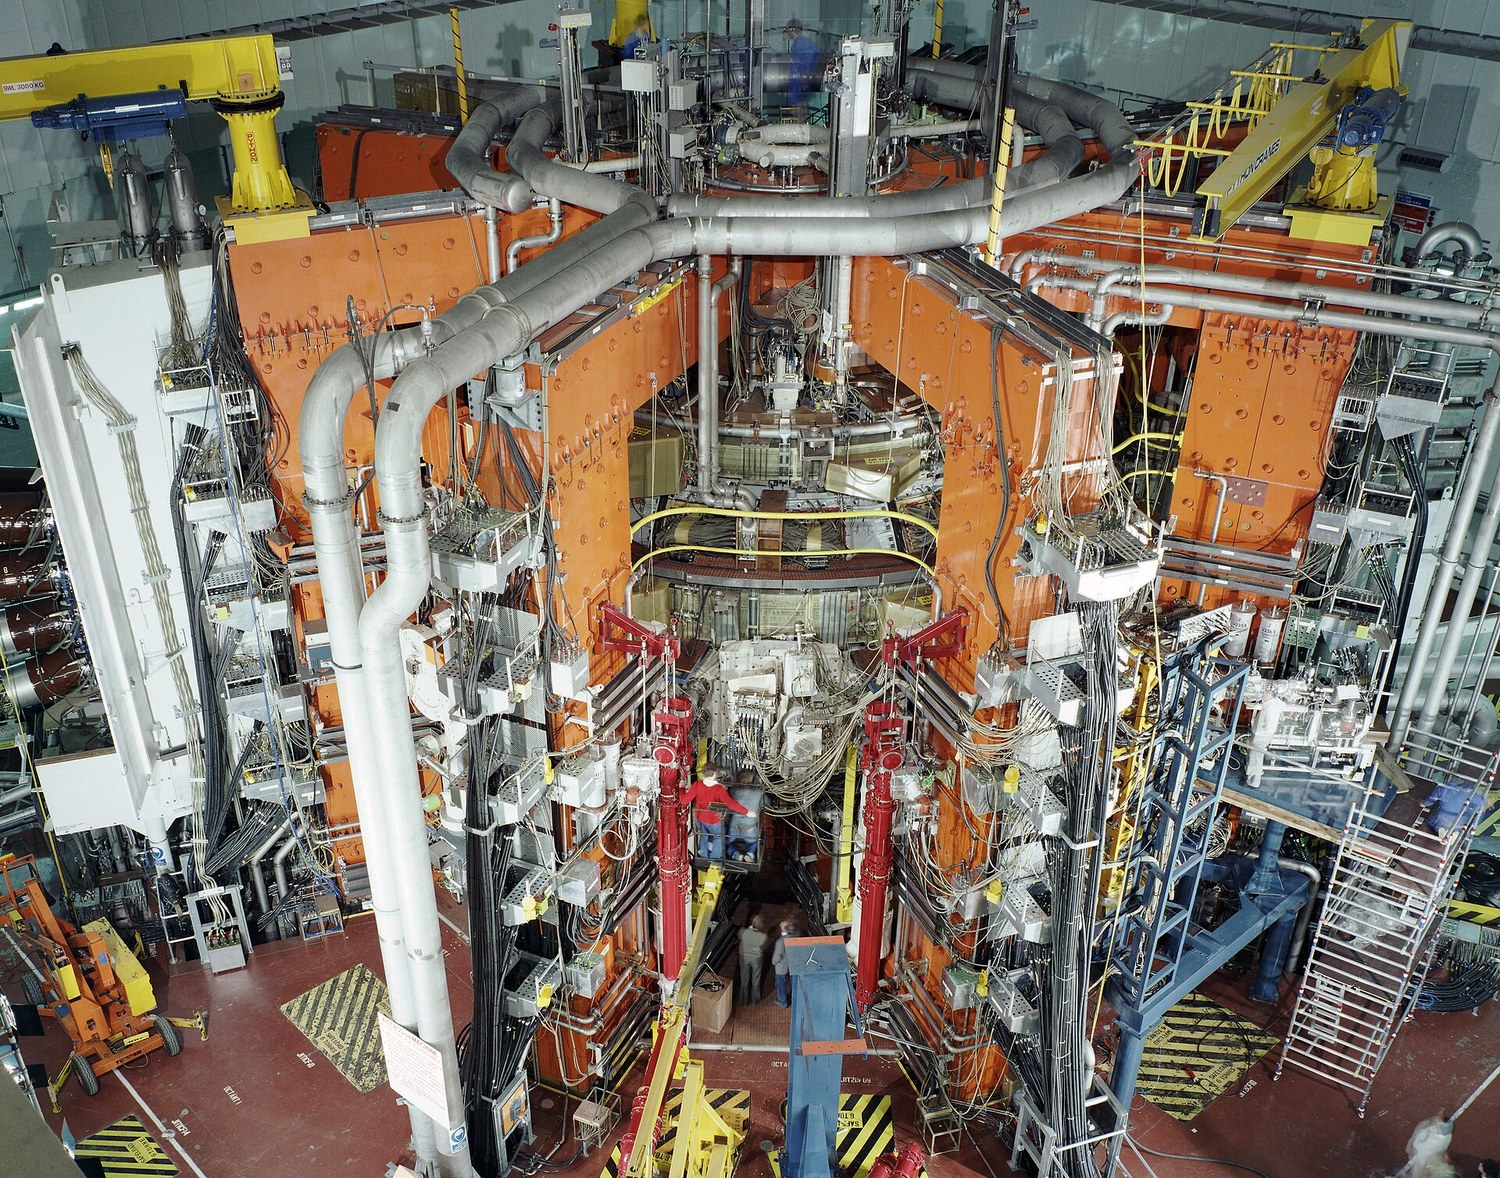
\includegraphics[width=0.72\textwidth]{../figures/w_jet_1991.jpg}
\caption{JET：第一次做氘氚实验的装置。本节 3.5 MeV 的 alpha 粒子，最早就是在 JET 的氘氚放电里成批出现的——从那时起，「自加热」不再是纸面上的项。}
\label{fig:photo-appw2}
\figsource{EFDA JET，CC BY-SA 3.0（Wikimedia Commons）}
\end{figure}

\section{出生：3.5 MeV 的 alpha 粒子是怎么来的}
\label{sec:app-w-birth}

前面几本账都把 alpha 粒子当成一行功率：附录 U 里是 $P_\alpha=111.3\ \mathrm{MW}$，
附录 V 里是「逃逸电子之外的另一类高能粒子」。可是这一行功率背后是一群\textbf{真实的粒子}：
每一次 D--T 反应生出一个带 $3.5\ \mathrm{MeV}$ 的 alpha 粒子。它的速度是光速的
$4\%$，回旋半径是 $5\ \mathrm{cm}$，出生位置离壁可能只有几十厘米。

沿用附录 S 与附录 U 的 D1（ITER 量级）工作点：$n=10^{20}\ \mathrm{m^{-3}}$、
$T=9.194\ \mathrm{keV}$、$B=5.3\ \mathrm{T}$、$a=2.0\ \mathrm{m}$、$R=6.2\ \mathrm{m}$；
聚变功率 $P_{\mathrm{fus}}=556.5\ \mathrm{MW}$，其中 alpha 分到五分之一。D--T 反应的
能量账是固定的：$17.6\ \mathrm{MeV}$ 里中子拿 $14.1\ \mathrm{MeV}$、alpha 拿
$3.5\ \mathrm{MeV}$，所以 alpha 的功率份额永远是 $1/5$。

\begin{equation}
P_\alpha = \frac{P_{\mathrm{fus}}}{5} = 111.3\ \mathrm{MW}, \qquad
E_{\alpha 0} = 3.5\ \mathrm{MeV} = 5.6076\times10^{-13}\ \mathrm{J}
\label{eq:app-w-birth}
\end{equation}

出生速度由 $E=\frac12 m_\alpha v^2$ 定：

\begin{equation}
v_{\alpha 0} = \sqrt{\frac{2E_{\alpha 0}}{m_\alpha}}
= 1.2992\times10^{7}\ \mathrm{m/s} = 0.0433\,c
\label{eq:app-w-gyro}
\end{equation}

这个速度决定了 alpha 的轨道有多大。带电粒子在磁场里回旋，半径
$\rho=mv/(qB)$；alpha 带 $2e$、质量是 $4\ \mathrm{u}$：

\begin{equation}
\rho_\alpha = \frac{m_\alpha v_{\alpha 0}}{Z_\alpha e B}
= 5.08\ \mathrm{cm} = 0.0508\ \mathrm{m}
\label{eq:app-w-rho}
\end{equation}

同样温度下氘离子的回旋半径是 $\rho_i=3.70\ \mathrm{mm}$。\textbf{alpha 的轨道比背景离子
大 $13.7$ 倍}。这不是细节：一个 alpha 粒子不是「长在」一根磁力线上，出生以后会横跨
好几厘米的磁面。

每秒有多少个 alpha 粒子出生？把功率除以单个粒子的能量：

\begin{equation}
S_\alpha = \frac{P_\alpha}{E_{\alpha 0}} = 1.9848\times10^{20}\ \mathrm{s^{-1}},
\qquad
\frac{S_\alpha}{V} = 2.3850\times10^{17}\ \mathrm{m^{-3}\,s^{-1}}
\label{eq:app-w-source}
\end{equation}

$V=832.2\ \mathrm{m^3}$ 是等离子体体积。\textbf{每秒钟有两千亿亿个 $3.5\ \mathrm{MeV}$ 的
粒子在芯部出生}。下一个问题是：这些粒子要把能量交给背景等离子体，而背景等离子体有没有
能力把它们拦下来？

\begin{table}[htbp]
\centering
\caption{一个 alpha 粒子的一生。四行不是四个事件，而是同一笔能量账在四个时间尺度上的
展开：出生是一瞬间，交出去要一秒，而打到壁上只需要半圈轨道。}
\label{tab:app-w-life}
\begin{tabular}{@{}p{2.5cm}p{3.0cm}p{3.6cm}p{3.6cm}@{}}
\hline
阶段 & 时间尺度 & 粒子在做什么 & 能量在谁手里 \\
\hline
出生 & $0$ & D--T 反应给出 $3.5\ \mathrm{MeV}$ 的 alpha &
全部在 alpha 身上（$5.6076\times10^{-13}\ \mathrm{J}$） \\
慢化 & $0.1627\ \mathrm{s}$（能量 e 折） &
沿轨道飞行，与电子、离子反复碰撞 & 逐步转给背景电子 \\
热化 & $0.8902\ \mathrm{s}$ &
速度掉到与背景离子同量级 & 与背景离子共享 \\
去向 & 之后 & 变成「热 alpha」或已经打到壁上 &
与背景完全混合，成为杂质与稀释源 \\
\hline
\end{tabular}

\end{table}

\begin{tip}{慢化是「换手」，不是「刹车」}{tip-app-w-oneway}
慢化常被想成 alpha 粒子「被挡住了」，其实不是：alpha 一路飞行，把能量一小口一小口转给
背景\textbf{电子}（大部分能量区间由电子阻力主导），自己越来越慢。被「挡住」的是能量：
能量留下来加热等离子体，粒子本身最后变成背景的一部分。
\end{tip}

{\footnotesize
\textbf{出处：} D--T 反应的 $17.6\ \mathrm{MeV}$ 能量分配与 alpha 功率份额 $1/5$ 参照
Wesson \textit{Tokamaks}（第 4 版，2011，第 1 章）与 Freidberg \textit{Plasma Physics
and Fusion Energy}（2007，第 1、13 章）。
回旋半径与特征时间的量级划分参照
Wesson 同书第 2 章。本节的数值口径（$P_{\mathrm{fus}}=556.5\ \mathrm{MW}$、
$V=832.2\ \mathrm{m^3}$）与附录 U 的 D1 工作点一致，全部由 \texttt{tools/\allowbreak{}calc/\allowbreak{}appW\_calc.py}
复算。
}

\section{慢化：为什么不能用「快离子」公式}
\label{sec:app-w-slowing}

教科书上有一个漂亮的公式，专门描述「快离子在等离子体里损失能量」：

\begin{equation}
\left.\frac{\diff E}{\diff x}\right|_{\text{快离子}}
= \frac{4\pi n_e Z^2 e^4 \ln\Lambda}{(4\pi\eps_0)^2 m_e v^2}
\label{eq:app-w-fastformula}
\end{equation}

它假设\textbf{快离子的速度远大于背景电子热速度} $v\gg v_{Te}$。把它代进 $3.5\ \mathrm{MeV}$
的 alpha，会得到一个毫秒量级的慢化时间。\textbf{这个答案是错的，而且错三个数量级。}

原因很简单：先算一下速度比。$T=9.194\ \mathrm{keV}$ 时电子热速度
$v_{Te}=\sqrt{2T/m_e}=5.6869\times10^{7}\ \mathrm{m/s}$，而 alpha 的出生速度只有
$1.2992\times10^{7}\ \mathrm{m/s}$：

\begin{equation}
x \equiv \frac{v_{\alpha 0}}{v_{Te}} = 0.2284 \;<\; 1
\label{eq:app-w-xratio}
\end{equation}

\textbf{alpha 比背景电子慢。} 式 \eqref{eq:app-w-fastformula} 的前提在这里不成立。正确的做法
是用一般的 Chand\-ra\-sekhar 阻力函数：一个速度为 $v$ 的试验粒子，在速度为 $v_{Tf}$ 的
场粒子背景中受到的阻力是

\begin{equation}
\vect{F} = -\frac{4\pi n_f Z_t^2 Z_f^2 e^4 \ln\Lambda}{(4\pi\eps_0)^2 m_f}\,
\frac{H(x)}{v^2}\,\unitvec{v}, \qquad
H(x) = \mathrm{erf}(x) - \frac{2x}{\sqrt{\pi}}\ee^{-x^2}, \quad x=\frac{v}{v_{Tf}}
\label{eq:app-w-chandrasekhar}
\end{equation}

关键在于 $H(x)$ 的形状：$x\gg1$ 时 $H\to1$（就是式 \eqref{eq:app-w-fastformula} 的
情形）。$x\ll1$ 时 $H\approx 4x^3/(3\sqrt{\pi})$。\textbf{阻力与速度成正比}，
而不是与 $v^{-2}$ 成正比。$x=0.2284$ 处精确值 $H=0.00869311$ 、渐近式
$4x^3/(3\sqrt{\pi})=0.00896879$，两者差 $3\%$，说明已经落在\textbf{线性阻力段}。

线性段的后果是干净利落的：阻力 $\vect{F}=-K\vect{v}$，速度按指数衰减，

\begin{equation}
K = \frac{16\sqrt{\pi}}{3}\cdot\frac{n_e Z_\alpha^2 e^4 \ln\Lambda}
{(4\pi\eps_0)^2 m_e v_{Te}^3} = 2.0421\times10^{-26}\ \mathrm{kg/s},
\qquad
\frac{\diff v}{\diff t} = -\frac{v}{\tau_v},\quad
\tau_v=\frac{m_\alpha}{K}=0.3254\ \mathrm{s}
\label{eq:app-w-tauv}
\end{equation}

能量按 $E\propto v^2$ 衰减，所以能量的 e 折时间只有速度的一半：$\tau_E=m_\alpha/(2K)
=0.1627\ \mathrm{s}$。这个数字可以独立验证。等离子体物理里还有一个「电子-离子能量
均分时间」，对 $n_e=10^{20}\ \mathrm{m^{-3}}$、$T=9.194\ \mathrm{keV}$ 用 NRL 公式算得
$\tau_{eq}=0.1638\ \mathrm{s}$，与 $\tau_E$ 之比是 $1.007$。\textbf{两条完全不同的推导路径
给出同一个数}，这本身就是「线性阻力段」判断正确的证据。

慢化到什么时候算完？当 alpha 的速度掉到与背景离子热速度相当时，它就不再是「快粒子」
而是背景的一部分了。氘离子热速度 $v_{th,i}=8.424185\times10^{5}\ \mathrm{m/s}$，于是

\begin{equation}
t_{\text{therm}} = \tau_v \ln\frac{v_{\alpha 0}}{v_{th,i}} = 0.8902\ \mathrm{s}
\label{eq:app-w-therm}
\end{equation}

只有 $2.74$ 个速度 e 折。\textbf{不到一秒}。所以「alpha 慢化时间约 1 秒」这个常被引用的
说法，在 D1 这样的参数下是对的，而它之所以对，恰恰是因为第一步就把 $x<1$ 认了出来。

沿途 alpha 会损失能量、也会在离子身上损失能量。两者的分界是一个临界能量。当
$v>v_c$ 时电子阻力占优（能量主要给电子，这对加热是好事）；$v<v_c$ 时离子阻力占优
（能量给了离子，而且此时 alpha 已经接近背景，加热效率下降）。把两段阻力相等写出来，
解出

\begin{equation}
\begin{aligned}
v_c^3 &= \frac{C_i}{K}, \qquad
C_i = \frac{4\pi n_i Z_\alpha^2 e^4 \ln\Lambda}{(4\pi\eps_0)^2 m_i}
= 1.095605\times10^{-6},\\
v_c &= 3.7716\times10^{6}\ \mathrm{m/s}, \qquad
E_c = \tfrac12 m_\alpha v_c^2 = 295.0\ \mathrm{keV}
\end{aligned}
\label{eq:app-w-vc}
\end{equation}

$295\ \mathrm{keV}$ 是 $32.08\,T_e$，也是出生能量的 $8.4\%$。文献里常引的
「alpha 临界能量 $0.3$--$0.5\ \mathrm{MeV}$」就是这个数。\textbf{它随温度变化}，温度越高
临界能量越高。

\begin{table}[htbp]
\centering
\caption{慢化的全部关键量。第二行是本节的判据：$x=0.2284$ 把问题从「快离子」改成
「线性阻力」，只这一处判断就决定后面所有时间尺度。}
\label{tab:app-w-slowing}
\begin{tabular}{@{}p{3.0cm}p{2.4cm}p{3.2cm}p{4.0cm}@{}}
\hline
量 & 数值 & 公式 & 说明 \\
\hline
$v_{\alpha 0}/v_{Te}$ & $0.2284$ & $v_{Te}=\sqrt{2T_e/m_e}$ &
小于 1，故\textbf{不能用}快离子公式 \\
$H(x)$ 精确 / 渐近 & $0.00869311$ / $0.00896879$ & $4x^3/(3\sqrt{\pi})$ &
差 $3\%$，落在线性阻力段 \\
阻力系数 $K$ & $2.0421\times10^{-26}\ \mathrm{kg/s}$ &
$K$ 的定义见式 \eqref{eq:app-w-tauv} &
$\vect{F}=-K\vect{v}$ \\
速度 e 折 $\tau_v$ & $0.3254\ \mathrm{s}$ & $m_\alpha/K$ & — \\
能量 e 折 $\tau_E$ & $0.1627\ \mathrm{s}$ & $m_\alpha/(2K)$ &
与 NRL 均分时间 $0.1638\ \mathrm{s}$ 相差 $0.7\%$ \\
热化时间 & $0.8902\ \mathrm{s}$ & $\tau_v\ln(v_{\alpha 0}/v_{th,i})$ &
$2.74$ 个速度 e 折 \\
临界能量 $E_c$ & $295.0\ \mathrm{keV}$ & $\frac12 m_\alpha(C_i/K)^{2/3}$ &
$32.08\,T_e$，出生能量的 $8.4\%$ \\
慢化路径 & $4.2272\times10^{6}\ \mathrm{m}$ & $v_{\alpha 0}\tau_v$ &
$4227\ \mathrm{km}$，绕环 $108514$ 圈 \\
\hline
\end{tabular}

\end{table}

慢化路径那一行值得单独看一眼：$v_{\alpha 0}\tau_v=4.2272\times10^{6}\ \mathrm{m}$，
也就是 $4227$ 公里。环向周长只有 $2\pi R=38.9557\ \mathrm{m}$，所以一个 alpha 粒子
在慢化完之前要\textbf{绕环运行约 $108514$ 圈}。这解释了两件事：第一，alpha 加热沿磁面
（极向与环向）几乎是均匀的；第二，它横跨磁面的距离却只有轨道宽度那么多。下一节算。

\begin{tip}{0.89 秒与 108514 圈：快粒子的两个尺度必须分开}{tip-app-w-locality}
「绕环 10 万圈」和「横向只走 18 厘米」听起来矛盾，其实不矛盾：粒子沿磁力线的运动是
自由的（平行方向没有磁场力），横跨磁面的运动是被磁场冻结的。慢化时间决定它\textbf{在磁面上
走多远}，轨道宽度决定它\textbf{跨过几个磁面}。加热的局域性由后者决定，不是前者。
\end{tip}

{\footnotesize
\textbf{出处：} Chand\-ra\-sekhar 阻力函数与 $H(x)$ 的形式参照 Chand\-ra\-sekhar
\textit{Principles of Stellar Dynamics}（1943）与 Spitzer \textit{Physics of Fully
Ionized Gases}（第 2 版，1962，第 5 章）。
临界能量的定义与「$0.3$--$0.5\ \mathrm{MeV}$」
量级参照 Wesson \textit{Tokamaks}（第 4 版，2011，第 2、9 章）与
Freidberg \textit{Plasma Physics and Fusion Energy}（2007，第 13 章）。
电子-离子
能量均分时间的 NRL 形式参照 NRL \textit{Plasma Formulary}（2013，第 1 章）。
本节全部数值由 \texttt{tools/\allowbreak{}calc/\allowbreak{}appW\_calc.py} 复算，其中 $\tau_{eq}$ 与 $\tau_E$ 的
闭合是独立的交叉验证。
}

\begin{figure}[htbp]
\centering
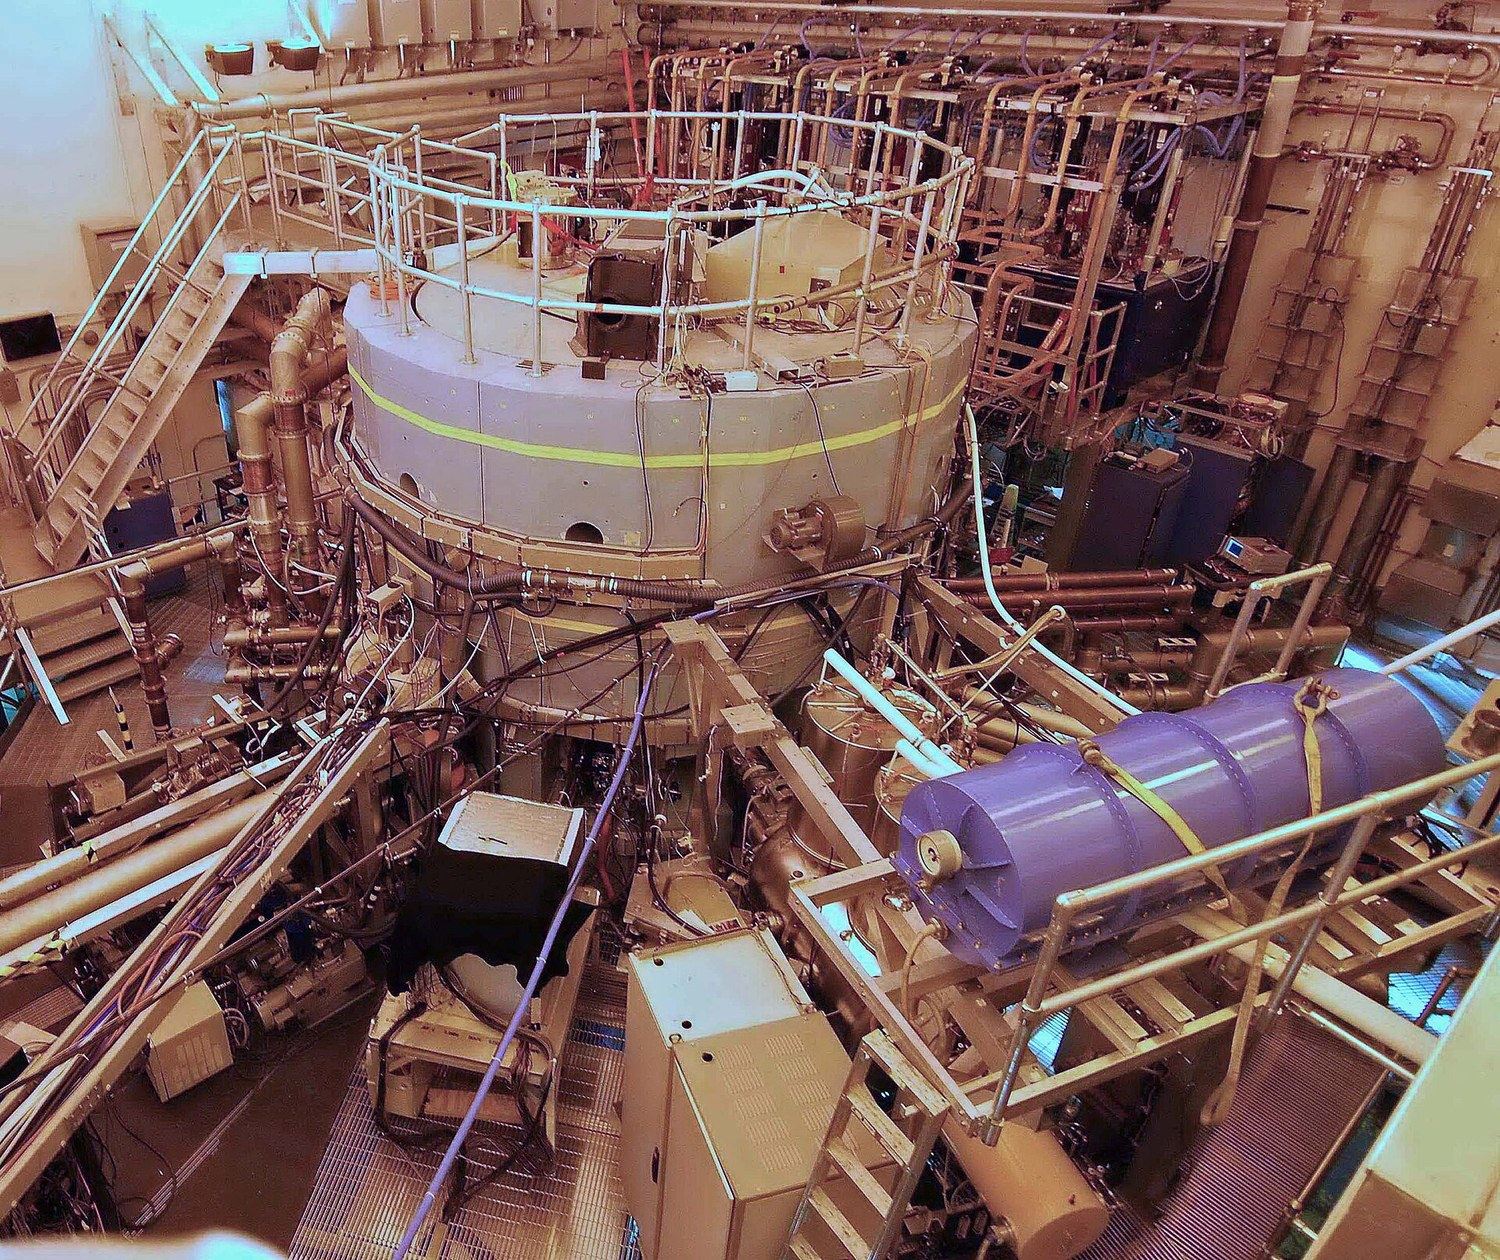
\includegraphics[width=0.78\textwidth]{../figures/w_cmod_cell.jpg}
\caption{Alcator C-Mod 的机厅：射频加热把能量送进等离子体，同时也把少数离子加速到兆电子伏量级——这些快离子就是本节的主角。它们的慢化长度，决定了加热到底落在多宽的一层里。}
\label{fig:photo-appw3}
\figsource{Jim Irby / MIT PSFC，CC BY 3.0（Wikimedia Commons）}
\end{figure}

\section{加热落在哪：18 厘米的径向宽度}
\label{sec:app-w-orbit}

慢化路径 $4227$ 公里说明 alpha 沿磁面跑得足够远，可以把加热抹匀；但「沿磁面均匀」
不等于「处处均匀」。\textbf{径向}是不抹的。原因是磁场约束只作用在垂直方向。一个 alpha
粒子虽然被绑在磁力线上，但它绕磁力线回旋、又沿磁力线来回弹跳，合成运动的径向投影
就是极向回旋半径

\begin{equation}
\rho_\theta = \frac{q\,\rho_\alpha}{\sqrt{\eps}}, \qquad \eps=\frac{a}{R}=0.322581,
\qquad \rho_\theta = 0.1790\ \mathrm{m} = 8.95\%\,a
\label{eq:app-w-rhotheta}
\end{equation}

完整香蕉轨道的宽度是它的两倍，$\Delta_\alpha=2\rho_\theta=0.3580\ \mathrm{m}$。也就是说
\textbf{一个 alpha 粒子出生以后，横跨磁面的活动范围约 $18$ 厘米}（半个香蕉宽度），
而整个等离子体半径是 $200$ 厘米。加热的径向分辨率就是这个数，不是 $\rho_\alpha=5\ \mathrm{cm}$，
也不是等离子体半径。

这个宽度立刻带来一个损失通道：如果粒子出生在离边界不到 $18$ 厘米的地方，它的轨道
就会有一部分落在等离子体外，也就是\textbf{第一次绕行就撞到壁上}。要算这份损失有多大，
需要知道出生率在半径上怎么分布。聚变反应率正比于 $n_Dn_T\propto n^2$，取
$n\propto(1-\rho^2)$（$\rho=r/a$）则出生率 $\propto(1-\rho^2)^2$。要求
$r+\rho_\theta>a$，即

\begin{equation}
\frac{r}{a} > 1 - \frac{\rho_\theta}{a} = 0.9105,
\qquad
f_{\text{首轨}} = \frac{\int_{0.9105}^{1}(1-\rho^2)^2\rho\diff\rho}
{\int_{0}^{1}(1-\rho^2)^2\rho\diff\rho}
= 0.4999\%
\label{eq:app-w-prompt}
\end{equation}

$0.4999\%$ 的 alpha 在第一圈就丢失；换成功率是 $f_{\text{首轨}}P_\alpha
=0.5564\ \mathrm{MW}$。\textbf{不到百分之一}，听起来可以忽略，但下一节会看到，它落在
第一壁上时的面积只有十几平方米，于是局部热流是 $0.0714\ \mathrm{MW/m^2}$：
不算致命，但足以在长脉冲里成为壁设计的输入之一。

\begin{table}[htbp]
\centering
\caption{轨道宽度与首次轨道损失。第 3 行是「加热落在哪」的答案：$18$ 厘米，
不是粒子的回旋半径，也不是等离子体半径。}
\label{tab:app-w-orbit}
\begin{tabular}{@{}p{2.7cm}p{2.6cm}p{3.0cm}p{4.2cm}@{}}
\hline
量 & 数值 & 公式 & 说明 \\
\hline
回旋半径 $\rho_\alpha$ & $0.0508\ \mathrm{m}$ & $m_\alpha v_{\alpha 0}/(Z_\alpha eB)$ &
是背景离子 $\rho_i=3.70\ \mathrm{mm}$ 的 $13.7$ 倍 \\
极向回旋半径 $\rho_\theta$ & $0.1790\ \mathrm{m}$ & $q\rho_\alpha/\sqrt{\eps}$ &
$8.95\%\,a$，\textbf{径向分辨率} \\
香蕉宽度 $\Delta_\alpha$ & $0.3580\ \mathrm{m}$ & $2\rho_\theta$ &
完整轨道横跨这么多磁面 \\
首轨损失边界 & $r/a>0.9105$ & $1-\rho_\theta/a$ &
出生率 $\propto(1-\rho^2)^2$ \\
首轨损失份额 & $0.4999\%$ & 见式 \eqref{eq:app-w-prompt} &
换成功率 $0.5564\ \mathrm{MW}$ \\
落点热流 & $0.0714\ \mathrm{MW/m^2}$ &
$\dfrac{0.5564\ \mathrm{MW}}{7.7911\ \mathrm{m^2}}$ &
落点面积按 $2\pi R\times0.2\ \mathrm{m}$ 估 \\
\hline
\end{tabular}

\end{table}

\begin{tip}{「沿磁面均匀」与「径向 18 厘米」不冲突}{tip-app-w-locality2}
这两句话说的是两个方向。沿磁面（极向 + 环向）是平行方向的自由运动，$0.89$ 秒里跑
$10$ 万圈，抹得比什么都匀；横跨磁面（径向）是垂直方向的漂移，慢化期间只能挪动
$18$ 厘米。所以 alpha 加热的真实图像是：\textbf{一层一层套着的薄壳}，每一层内部均匀，
层与层之间不均匀，而不是「芯部一个点热、其余都冷」。
\end{tip}

{\footnotesize
\textbf{出处：} 香蕉轨道宽度与极向回旋半径的定义参照 Wesson \textit{Tokamaks}
（第 4 版，2011，第 3 章）与 Freidberg \textit{Plasma Physics and Fusion Energy}
（2007，第 13 章）。
快粒子首次轨道损失与逃生锥的几何参照 Wesson 同书第 3 章与
Hender 等（2007）\textit{Nucl.\ Fusion} \textbf{47}, S128。出生率的
$(1-\rho^2)^2$ 剖面与 $18$ 厘米的落点宽度为本附录自拟的简化口径，量级 1 的系数
由 \texttt{tools/\allowbreak{}calc/\allowbreak{}appW\_calc.py} 复算。
}

\section{慢化分布与高能尾巴}
\label{sec:app-w-tail}

到上一节为止，我们跟着\textbf{一个} alpha 粒子走完了一生。现在把几亿亿个粒子放在一起看：
稳态下，每一时刻都有一批粒子处在不同的慢化阶段，它们组成一个速度分布。经典结果
（忽略扩散、只保留阻力）是

\begin{equation}
f(v) \propto \frac{1}{v^3+v_c^3}, \qquad v_{th,i} < v < v_{\alpha 0}
\label{eq:app-w-dist}
\end{equation}

这个分布的来历可以这样读：单位时间在 $v_{\alpha 0}$ 出生的粒子，要用
$\diff t/\diff v$ 的时间待在这个速度上，而线性阻力段里 $\diff v/\diff t=-v/\tau_v$，
再叠加上离子阻力在低速端的截断，就得到分母的 $v^3+v_c^3$。分布的两端行为完全
不同：$v\gg v_c$ 时 $f\propto v^{-3}$，是\textbf{重尾巴}；$v\ll v_c$ 时 $f\to$ 常数，
粒子堆在临界能量以下。

把这个分布对 $v\in[v_{th,i},v_{\alpha 0}]$ 积分，得到快 alpha 的平均能量

\begin{equation}
\langle E\rangle = \frac{\int \frac12 m_\alpha v^2\,f(v)v^2\diff v}
{\int f(v)v^2\diff v} = 1191.1\ \mathrm{keV} = 0.3403\,E_{\alpha 0}
\label{eq:app-w-meanE}
\end{equation}

\textbf{平均能量只有出生能量的三分之一}。因为尾巴很重、而粒子大部分时间待在低速端。
用这个平均值数密度和压强：

\begin{equation}
n_{\text{fast}} = \frac{S_\alpha}{V}\,t_{\text{therm}} = 2.1231\times10^{17}\ \mathrm{m^{-3}}
= 0.2123\%\,n_e, \qquad
p_{\text{fast}} = \frac{2}{3}n_{\text{fast}}\langle E\rangle
= 2.7011\times10^{4}\ \mathrm{Pa}
\label{eq:app-w-pfast}
\end{equation}

这里用 $p=(2/3)n\langle E\rangle$ 而不是 $nk_BT$：快粒子不是热平衡分布，压强来自
动能的 $2/3$，而不是温度的线性外推。对比热压 $p_{th}=2.9461\times10^{5}\ \mathrm{Pa}$，
快粒子贡献 $9.17\%$；折成 beta 是 $\beta_{\text{fast}}=0.241671\%$，占
$\beta_{\text{tot}}=2.6359\%$ 的同样是 $9.17\%$。\textbf{「alpha 只占百分之几」这句话
在这里第一次有了确切的数字}。它不是「可以忽略」，而是「和一套加热系统同量级」。
如果再叠上中性束与射频产生的快离子，这个份额还要往上走。

最后看尾巴。定义「尾巴」为 $v>2v_c$（也就是能量超过 $4E_c$）的粒子：

\begin{equation}
\frac{N_{v>2v_c}}{N_{\text{tot}}} = 41.2888\%, \qquad
\frac{W_{v>2v_c}}{W_{\text{tot}}} = 74.5395\%
\label{eq:app-w-tail}
\end{equation}

\textbf{四成的粒子带着七成半的能量。} 这一行数字是后面两节的钥匙：不稳定性由尾巴里
那些「快」的粒子驱动（它们速度接近 Alfvén 速度、能量足够共振）。壁上的热斑也
由尾巴造成（它们轨道最宽、最容易丢）。慢化分布不是一条尾巴挂在热分布上，而是
\textbf{尾巴里装着大部分能量}。

\begin{table}[htbp]
\centering
\caption{快 alpha 的宏观量与尾巴。表里每一行都只依赖上一节的 $\tau_v$ 与 $v_c$，
没有引入新的自由参数。}
\label{tab:app-w-tail}
\begin{tabular}{@{}p{3.2cm}p{2.6cm}p{2.9cm}p{3.6cm}@{}}
\hline
量 & 数值 & 公式 & 说明 \\
\hline
平均能量 $\langle E\rangle$ & $1191.1\ \mathrm{keV}$ &
定义式 \eqref{eq:app-w-meanE} & 只有出生能量的 $34.03\%$ \\
快 alpha 密度 & $2.1231\times10^{17}\ \mathrm{m^{-3}}$ &
$(S_\alpha/V)t_{\text{therm}}$ & 占电子密度 $0.2123\%$ \\
快 alpha 压强 & $2.7011\times10^{4}\ \mathrm{Pa}$ &
$(2/3)n_{\text{fast}}\langle E\rangle$ & 热压的 $9.17\%$ \\
$\beta_{\text{fast}}$ & $0.241671\%$ & $2\mu_0p_{\text{fast}}/B^2$ &
占 $\beta_{\text{tot}}=2.6359\%$ 的 $9.17\%$ \\
尾巴粒子份额 & $41.2888\%$ & $v>2v_c$ & 能量超过 $4E_c$ \\
尾巴能量份额 & $74.5395\%$ & $v>2v_c$ & \textbf{四成粒子带七成半能量} \\
\hline
\end{tabular}

\end{table}

\begin{tip}{「只占百分之几」不是「可以忽略」}{tip-app-w-fewpercent}
快 alpha 的密度只有电子的 $0.2\%$，很容易被当成小量。但单个 alpha 的能量是背景的 $130$ 倍
（$1191\ \mathrm{keV}$ 对 $9.2\ \mathrm{keV}$），合起来它们仍带热压的 $9\%$：
\textbf{密度小近 470 倍，压强只小 10 倍}。
判断一个群体重要不重要，要看它带的压强和自由能，不是看它的人数。附录 V 的逃逸电子
也是这个道理：电流占比小，破坏力最大。
\end{tip}

{\footnotesize
\textbf{出处：} 经典慢化分布 $f\propto 1/(v^3+v_c^3)$ 参照 Wesson \textit{Tokamaks}
（第 4 版，2011，第 9 章）与 Freidberg \textit{Plasma Physics and Fusion Energy}
（2007，第 13 章）。
快粒子压强用 $(2/3)n\langle E\rangle$ 的口径参照
Freidberg 同书第 13 章。
alpha 密度与 beta 份额的量级参照 Wesson 同书第 9 章。
本节的全部分布积分、平均值与尾巴份额由 \texttt{tools/\allowbreak{}calc/\allowbreak{}appW\_calc.py} 用
$400000$ 点梯形积分独立复算，不引用任何外部结论数值。
}

\section{快粒子驱动的不稳定性：先算三个比值}
\label{sec:app-w-instability}

有了「四成粒子带七成半能量」这个事实，不稳定性就不再意外：一个带自由能、又有速度
接近 Alfvén 速度的粒子群，正是波的不稳定驱动源。但在谈具体的模之前，先把\textbf{三个
无量纲比值}算出来。它们决定了哪些模能被驱动：

\begin{equation}
v_A = \frac{B}{\sqrt{\mu_0 n_i m_i}} = 7.3380\times10^{6}\ \mathrm{m/s},
\qquad
\frac{v_{\alpha 0}}{v_A} = 1.7705
\label{eq:app-w-va}
\end{equation}

alpha 是\textbf{超 Alfvén 的}（$1.77$ 倍）。这一个数就决定了 alpha 可以和剪切 Alfvén
波共振：共振条件是 $v_\parallel\approx v_A$，而 alpha 的速度分布在
$v_A$ 两侧都有（出生时 $1.77v_A$，慢化时穿过 $v_A$），所以\textbf{共振粒子总是存在}，
只要波的频率对得上。

第二组是频率对得对不对。环向 Alfvén 本征模（TAE）的频率由 Alfvén 速度和平行波数
决定，最简单的估计是

\begin{equation}
f_{\text{TAE}} = \frac{v_A}{4\pi qR},
\qquad f_{\text{TAE}}(q{=}1)=94.2\ \mathrm{kHz},\;
f_{\text{TAE}}(q{=}2)=47.09\ \mathrm{kHz},\;
f_{\text{TAE}}(q{=}3)=31.4\ \mathrm{kHz}
\label{eq:app-w-tae}
\end{equation}

而 alpha 的\textbf{环向进动}频率是另一个量级：

\begin{equation}
\omega_d = \frac{E}{Z_\alpha e B R^2} = 8589.72\ \mathrm{rad/s}
\;\Longrightarrow\; f_d = 1367.10\ \mathrm{Hz}
\label{eq:app-w-precess}
\end{equation}

超 Alfvén 粒子的\textbf{弹跳}频率介于两者之间：取 $r=1\ \mathrm{m}$、$q=2$，

\begin{equation}
f_b = \frac{1}{2\pi}\cdot\frac{v_{\alpha 0}}{qR}\sqrt{\frac{r}{2R}}
= 47.35\ \mathrm{kHz}
\label{eq:app-w-bounce}
\end{equation}

把三个频率排在一起：$f_d:f_b:f_{\text{TAE}}(q{=}2) = 1 : 34.6 : 34.4$。\textbf{弹跳频率与
TAE 频率几乎相等}。这不是巧合，而是超 Alfvén 粒子驱动 TAE 的条件本身。进动频率
比它们低三十多倍，正对应鱼骨模（内核 kink 与进动alpha 共振）。作为上限，离子回旋
频率 $f_{cD}=40.41\ \mathrm{MHz}$ 比这一切都高三个量级，所以这些模都是\textbf{低频
MHD 尺度的模}，流体描述仍然可用。

驱动强弱则由前面已经算好的两个比值给出：

\begin{equation}
\frac{\beta_{\text{fast}}}{\beta_{\text{tot}}} = 9.17\%,
\qquad
\frac{n_{\text{fast}}}{n_e} = 0.2123\%
\label{eq:app-w-ratios}
\end{equation}

这两个数合起来说明：驱动\textbf{不弱也不强}。它足以让模不稳定（实验室里
$\beta_{\text{fast}}/\beta_{\text{tot}}$ 到百分之几就足以激发 TAE），但离「快粒子
主导平衡」还差得远，所以预期的后果是\textbf{中等幅度的饱和}与增强的快粒子输运，而不是
整体崩溃。

\begin{table}[htbp]
\centering
\caption{三类快粒子不稳定性与它们对应的共振条件。\textbf{本表不给阈值}：阈值依赖
$q$ 剖面、快粒子分布的具体形状与阻尼机制，不是本附录的简化模型能定的；能给的是
「共振在哪里」和「驱动有多强」这两件事。}
\label{tab:app-w-instability}
\begin{tabular}{@{}p{2.5cm}p{2.4cm}p{3.1cm}p{3.6cm}@{}}
\hline
不稳定性 & 共振条件 & 本附录算出的对应量 & 后果 \\
\hline
鱼骨模 & $\omega\approx\omega_d$（进动共振） &
$f_d=1367.10\ \mathrm{Hz}$ & 芯部快粒子被抛出，$q=1$ 面附近重分布 \\
TAE／环向 Alfvén 模 & $v_\parallel\approx v_A$，$\omega\approx v_A/(2qR)$ &
$v_{\alpha 0}/v_A=1.7705$，$f_{\text{TAE}}(q{=}2)=47.09\ \mathrm{kHz}$ &
中等幅度饱和，快粒子径向输运增强 \\
alpha 连续谱／BAE & 弹跳与进动共振的连续带 &
$f_b=47.35\ \mathrm{kHz}$（$r=1\ \mathrm{m}$） &
取决于剖面，可能驱动也可能阻尼 \\
\hline
\end{tabular}

\end{table}

\begin{tip}{先算三个比值，再谈不稳定性}{tip-app-w-ratios}
快粒子不稳定性的教科书讨论容易出现两种毛病：一种是直接背模的名字（鱼骨、TAE、
BAE、EPM……），另一种是直接抄阈值。两种都不解决问题。可检验的做法是先把三个
\textbf{无量纲比值}算出来：$v_{\alpha 0}/v_A$（能不能共振）、$n_{\text{fast}}/n_e$
（有多少驱动粒子）、$\beta_{\text{fast}}/\beta_{\text{tot}}$（驱动相对平衡有多强）。
本节的三个数是 $1.7705$、$0.2123\%$、$9.17\%$；换一台装置、换一个温度，这三个数
会变，而判断的顺序不变。
\end{tip}

{\footnotesize
\textbf{出处：} TAE 的色散关系与「快粒子速度接近 $v_A$ 时共振」的判据参照
Wesson \textit{Tokamaks}（第 4 版，2011，第 9 章）与 Freidberg \textit{Plasma
Physics and Fusion Energy}（2007，第 13 章）。
鱼骨模与 alpha 进动共振的机理参照
Wesson 同书第 9 章与 Hender 等（2007）\textit{Nucl.\ Fusion} \textbf{47}, S128。
alpha 连续谱与 BAE 的定性描述参照 Wesson 同书第 9 章。本节所有频率与比值由
\texttt{tools/\allowbreak{}calc/\allowbreak{}appW\_calc.py} 复算，\textbf{不给出任何阈值数字}——这是刻意的口径声明，
理由写在表 \ref{tab:app-w-instability} 的题注里。
}

\section{损失与第一壁：三条通道}
\label{sec:app-w-loss}

快粒子对装置的第一项直接威胁是\textbf{局部热负荷}。要算它，得先分清有几条通道把 alpha
送到壁上。三条通道的物理完全不同，量级也不同：

\textbf{通道一：首次轨道损失。} 上一节已经算出 $f_{\text{首轨}}=0.4999\%$，也就是
$0.5564\ \mathrm{MW}$。这条通道的特征是\textbf{只和几何有关}：它取决于
$\rho_\theta/a=8.95\%$ 与出生率剖面，与不稳定性、与运行模式都无关。它也无法靠
「改善约束」消除。除非把等离子体做大或把 $q$ 降下来。

\textbf{通道二：纹波损失。} 环向场线圈是分立的，线圈之间的磁场比线圈处弱一点点，这个
不均匀叫纹波。设纹波幅度 $\delta=\Delta B/B=0.005$（$0.5\%$，现代托卡马克的典型
量级），那么被纹波「抓住」的粒子满足

\begin{equation}
\left|\frac{v_\parallel}{v}\right| < \sqrt{2\delta} = 0.1000
\label{eq:app-w-ripple}
\end{equation}

也就是速度方向落在赤道两侧 $\pm5.7^\circ$ 锥内的粒子会被纹波俘获并漂出。这部分立体角
占全部方向的 $0.50\%$。但被抓住的粒子不一定马上丢失。它们可能再被解俘获。工程上
的简化口径是「落入纹波损失锥的 alpha 有 $1\%$ 到 $3\%$ 真正丢失」，对应
$1.1130$ 到 $3.3390\ \mathrm{MW}$。\textbf{这条通道比首轨损失大两到六倍}，而且它随纹波
幅度变化，是可以靠线圈设计压下去的。

\textbf{通道三：不稳定性驱动的输运。} 上一节说的 TAE 与鱼骨模一旦饱和，会把
快粒子从芯部搬到边缘。这条通道的定量幅度依赖具体剖面与饱和机制，本附录的模型
算不出来。按表 \ref{tab:app-w-instability} 的口径，这里只声明它存在、并指出它
作用在\textbf{已经慢化了一段时间}的粒子上（因此能量较低、落点更宽）。

三条通道合起来的直接后果是壁上的\textbf{局部热流}。取首轨损失的落点面积
$2\pi R\times0.2\ \mathrm{m}=7.7911\ \mathrm{m^2}$，热流是

\begin{equation}
q_{\text{wall}} = \frac{0.5564\ \mathrm{MW}}{7.7911\ \mathrm{m^2}}
= 0.0714\ \mathrm{MW/m^2}
\label{eq:app-w-qwall}
\end{equation}

对比附录 N 的稳态靶板热流（$q_\perp$ 从几十 $\mathrm{MW/m^2}$ 被倾角压到个位数），
$0.0714\ \mathrm{MW/m^2}$ 小两个量级。\textbf{这不是设计驱动量}。但它是「点状」的：
如果某些 alpha 因为不稳定性集中打在一条带上，局部值会抬上去，而且它落在
\textbf{第一壁}而不是偏滤器靶板上，那里没有倾角、没有脱靶保护。所以正确的说法是：
\textbf{快粒子损失不是总能量问题，是分布问题。}

快 alpha 的分布怎么测？两条路：中性粒子分析器（NPA）接收电荷交换
产生的中性原子，反推快离子能量谱。快离子 D-alpha 光谱（FIDA）用沿视线收集的
巴尔末 alpha 线多普勒位移，反推快离子速度分布。两者的共同难点是\textbf{都要扣除
背景中性密度}这个不确定因子，和附录 Q 里探针诊断要扣离子电流是同一类问题。

\begin{table}[htbp]
\centering
\caption{快粒子损失的三条通道。第 3 行\textbf{故意留空}：本附录的简化模型给不出
不稳定性驱动的损失份额，宁可写「算不出」也不填一个编造的数字。}
\label{tab:app-w-loss}
\begin{tabular}{@{}p{2.4cm}p{2.7cm}p{3.2cm}p{3.5cm}@{}}
\hline
通道 & 损失份额 / 功率 & 物理机制 & 可否靠设计改善 \\
\hline
首次轨道损失 & $0.4999\%$ / $0.5564\ \mathrm{MW}$ &
$\rho_\theta/a=8.95\%$，出生在 $r/a>0.9105$ 的粒子首圈丢失 &
只能靠加大尺寸或降低 $q$ \\
纹波损失 & $1\%$--$3\%$ / $1.1130$--$3.3390\ \mathrm{MW}$ &
$\sqrt{2\delta}=0.1000$ 的纹波俘获锥 & 可以：减小 $\delta$、优化线圈 \\
不稳定性输运 & 未定量（模型算不出） &
TAE／鱼骨模饱和后把已慢化的粒子搬到边缘 & 可以：控制剖面与 $q$ \\
\hline
落点热流 & $0.0714\ \mathrm{MW/m^2}$ &
$0.5564\ \mathrm{MW}$ 摊在 $7.7911\ \mathrm{m^2}$ 上 &
不是总量问题，是分布问题 \\
\hline
\end{tabular}

\end{table}

\begin{tip}{把「算不出」写在表里}{tip-app-w-honest}
读者会注意到表 \ref{tab:app-w-loss} 的第三行没有数字。这是刻意留的：不稳定性驱动的
输运份额需要非线性饱和模型，而本附录用的是「经典慢化 + 轨道宽度」这一套可手算的
工具，它做不到。\textbf{把做不到的地方标出来，比用一个看起来精确的数字盖过去更有用}。
因为前者的误差是已知的、可继续追击的，后者的误差是隐藏的。全书的口径在附录 V 的
「把简化声明写在明处」里已经立过一次，这里是第二次。
\end{tip}

{\footnotesize
\textbf{出处：} 纹波俘获条件 $|v_\parallel/v|<\sqrt{2\delta}$ 与纹波损失的量级参照
Wesson \textit{Tokamaks}（第 4 版，2011，第 3 章）与 Hender 等（2007）
\textit{Nucl.\ Fusion} \textbf{47}, S128。
首次轨道损失与壁热负荷的量级参照
Wesson 同书第 3 章。
NPA 与 FIDA 的原理参照 Hutchinson \textit{Principles of Plasma
Diagnostics}（2002，第 7、11 章）。本节凡标出数字的量都由
\texttt{tools/\allowbreak{}calc/\allowbreak{}appW\_calc.py} 复算。
不稳定性输运份额明确留空。
}

\section{六道估算练习}
\label{sec:app-w-problems}

\textbf{练习 1（出生与回旋半径）}
D--T 反应给出 $3.5\ \mathrm{MeV}$ 的 alpha。求它的速度、在 $B=5.3\ \mathrm{T}$ 中的
回旋半径，并与同温度下氘离子的回旋半径比较。

\textbf{解答}：$E_{\alpha 0}=3.5\ \mathrm{MeV}=5.6076\times10^{-13}\ \mathrm{J}$，
由式 \eqref{eq:app-w-gyro} 得 $v_{\alpha 0}=1.2992\times10^{7}\ \mathrm{m/s}
=0.0433\,c$；由式 \eqref{eq:app-w-rho} 得 $\rho_\alpha=0.0508\ \mathrm{m}=5.08\ \mathrm{cm}$。
氘离子在 $T=9.194\ \mathrm{keV}$ 时 $\rho_i=3.70\ \mathrm{mm}$，比值 $13.7$。\textbf{要点}：
这个比值不是「alpha 更热所以更大」这么简单。它同时来自质量大 $2$ 倍（$\rho\propto\sqrt{m}$）
和电荷多 $1$ 倍（$\rho\propto1/Z$），合起来 $\sqrt{2}/1\times\sqrt{3.5\ \mathrm{MeV}/9.194\ \mathrm{keV}}$
的主要贡献其实是能量比。

\textbf{练习 2（慢化时间与适用条件）}
先用「快离子」公式估计 $3.5\ \mathrm{MeV}$ alpha 在 $n_e=10^{20}\ \mathrm{m^{-3}}$、
$T=9.194\ \mathrm{keV}$ 中的慢化时间；再检查它是否适用，并给出正确的时间尺度。

\textbf{解答}：电子热速度 $v_{Te}=5.6869\times10^{7}\ \mathrm{m/s}$，而
$v_{\alpha 0}=1.2992\times10^{7}\ \mathrm{m/s}$，比值 $x=0.2284<1$。
式 \eqref{eq:app-w-fastformula} 的前提\textbf{不成立}。改用线性阻力段：$K=2.0421\times10^{-26}\ \mathrm{kg/s}$，
$\tau_v=m_\alpha/K=0.3254\ \mathrm{s}$、$\tau_E=m_\alpha/(2K)=0.1627\ \mathrm{s}$，
热化时间 $t_{\text{therm}}=\tau_v\ln(v_{\alpha 0}/v_{th,i})=0.8902\ \mathrm{s}$。
\textbf{要点}：把「快」当成一个绝对判断是错的；快不快是相对\textbf{背景电子}说的。

\textbf{练习 3（临界能量）}
求 alpha 的临界能量 $E_c$，并说明它为什么随温度变化。

\textbf{解答}：$C_i=1.095605\times10^{-6}$，$v_c^3=C_i/K$ 给
$v_c=3.7716\times10^{6}\ \mathrm{m/s}$，$E_c=\frac12m_\alpha v_c^2=295.0\ \mathrm{keV}
=32.08\,T_e$。\textbf{要点}：$v_c$ 来自电子阻力与离子阻力相等，而电子阻力正比于
$n_e/v_{Te}^3\propto n_e T_e^{-3/2}$；温度升高时电子阻力下降，交点右移，所以
$E_c\propto T_e$。文献里「$0.3$--$0.5\ \mathrm{MeV}$」对应的是更热的等离子体。

\textbf{练习 4（首次轨道损失）}
取 $q=2$、$\eps=a/R=0.322581$、$\rho_\alpha=0.0508\ \mathrm{m}$，求极向回旋半径，
并估计首次轨道损失的份额与功率。

\textbf{解答}：$\rho_\theta=q\rho_\alpha/\sqrt{\eps}=0.1790\ \mathrm{m}=8.95\%\,a$。
出生率 $\propto(1-\rho^2)^2$、边界 $r/a>1-\rho_\theta/a=0.9105$，积分得
$f_{\text{首轨}}=0.4999\%$，功率 $0.4999\%\times111.3\ \mathrm{MW}=0.5564\ \mathrm{MW}$。
\textbf{要点}：份额这么小是因为 $\rho_\theta$ 只有半径的 $9\%$，而出生率在边缘是零；
但注意份额对 $q$ 是一次方敏感（$\rho_\theta\propto q$）。

\textbf{练习 5（快粒子压强）}
已知 $\langle E\rangle=1191.1\ \mathrm{keV}$、$t_{\text{therm}}=0.8902\ \mathrm{s}$、
$S_\alpha/V=2.3850\times10^{17}\ \mathrm{m^{-3}s^{-1}}$，求快 alpha 的密度、压强与
beta 份额，并与热压比较。

\textbf{解答}：$n_{\text{fast}}=(S_\alpha/V)t_{\text{therm}}=2.1231\times10^{17}\ \mathrm{m^{-3}}
=0.2123\%\,n_e$；$p_{\text{fast}}=(2/3)n_{\text{fast}}\langle E\rangle
=2.7011\times10^{4}\ \mathrm{Pa}$；$p_{th}=2.9461\times10^{5}\ \mathrm{Pa}$，比值 $9.17\%$；
$\beta_{\text{fast}}=0.241671\%$ 占 $\beta_{\text{tot}}=2.6359\%$ 的 $9.17\%$。
\textbf{要点}：注意压强用的是 $(2/3)n\langle E\rangle$ 而不是 $nk_BT$。快粒子不在热平衡上。

\textbf{练习 6（频率对比）}
求 $v_A$、$f_{\text{TAE}}(q=2)$、$f_d$（进动）与 $f_b$（$r=1\ \mathrm{m}$），
排出它们的比值，并解释哪一对频率的接近决定了 TAE 的驱动。

\textbf{解答}：$v_A=B/\sqrt{\mu_0n_im_i}=7.3380\times10^{6}\ \mathrm{m/s}$，故
$v_{\alpha 0}/v_A=1.7705$；阿尔法连续谱频率 $f_{\text{TAE}}=v_A/(4\pi qR)$，代入得
$47.09\ \mathrm{kHz}$；进动频率 $\omega_d=E/(Z_\alpha eBR^2)=8589.72\ \mathrm{rad/s}$，即
$f_d=1367.10\ \mathrm{Hz}$；弹跳频率 $f_b$ 由 $v_{\alpha 0}/(qR)\sqrt{r/(2R)}/(2\pi)$
给出，为 $47.35\ \mathrm{kHz}$。三者比值
$f_d:f_b:f_{\text{TAE}}=1:34.6:34.4$。\textbf{要点}：$f_b\approx f_{\text{TAE}}$ 是 TAE 被
超 Alfvén 粒子驱动的条件；$f_d$ 比它们低三十多倍，对应的是鱼骨模的进动共振。

\section{来源、分级与版权说明}
\label{sec:app-w-source}

\begingroup\small
本附录使用的公式类型、结论与题型均有明确出处；所有数值、表格与文字自拟，并由
仓库脚本 \texttt{tools/\allowbreak{}calc/\allowbreak{}appW\_calc.py} 独立复算（印刷精度与脚本输出逐位一致）。

\textbf{三档难度标记：}
(1) 带 $\star$ 的内容只需要第 3 章（单粒子轨道）与第 8 章（碰撞与输运）——
例如回旋半径、慢化时间、首次轨道损失。
(2) 带 $\star\star$ 的内容还要第 7 章（动理学）与第 9 章（不稳定性）——
例如慢化分布、快粒子压强、TAE 频率。
(3) 带 $\star\star\star$ 的内容涉及非线性饱和与输运，本附录\textbf{只给判据、不给数字}——
例如不稳定性驱动的损失份额。

\begin{table}[htbp]
\centering
\caption{本附录的借鉴来源与自拟部分对照表。所有量级 1 的精确系数、实验定标与工程设计
值均为本附录自拟；故只给书名、作者、年份、章节或卷期页。}
\label{tab:app-w-source}
\begin{tabular}{@{}p{1.4cm}p{5.4cm}p{4.0cm}p{3.4cm}@{}}
\hline
节 & 借鉴了什么（结论 / 公式形式 / 题型） & 出处 & 本附录自拟的部分 \\
\hline
W.1 & D--T 能量分配、alpha 功率份额、回旋半径量级 &
Wesson \textit{Tokamaks} 第 4 版第 1、2 章；Freidberg 2007 第 1、13 章 &
全部数值、生命周期的四阶段划分与表 W.1 \\
W.2 & Chand\-ra\-sekhar 阻力函数、临界能量、均分时间 NRL 形式 &
Chand\-ra\-sekhar 1943 第 5 章；Spitzer 1962 第 5 章；NRL Formulary 2013 第 1 章 &
$x=0.2284$ 的适用性判断、$K$ 与 $\tau_v$ 的写法、$\tau_{eq}$ 闭合验证 \\
W.3 & 香蕉轨道宽度、极向回旋半径、逃生锥几何 &
Wesson 第 4 版第 3 章；Hender 等 2007 &
$(1-\rho^2)^2$ 出生剖面、$0.2\ \mathrm{m}$ 落点宽度、$0.0714\ \mathrm{MW/m^2}$ \\
W.4 & 慢化分布 $1/(v^3+v_c^3)$、$(2/3)n\langle E\rangle$ 口径 &
Wesson 第 4 版第 9 章；Freidberg 2007 第 13 章 &
分布积分、$1191.1\ \mathrm{keV}$ 与 $9.17\%$、尾巴的两行份额 \\
W.5 & TAE 色散关系、鱼骨模与进动共振、alpha 连续谱定性 &
Wesson 第 4 版第 9 章；Hender 等 2007 &
三个频率的具体数值、三个无量纲比值、\textbf{不给阈值}的口径 \\
W.6 & 纹波俘获条件、NPA 与 FIDA 原理 &
Wesson 第 4 版第 3 章；Hutchinson 2002 第 7、11 章 &
三条通道的划分、$1\%$--$3\%$ 简化口径、热流与留空的第三行 \\
\hline
\end{tabular}

\end{table}

\textbf{三条「不复制」约定：}
(1) 不复制任何教材或论文的表格数值——本附录每一张表的数字都能用
\texttt{tools/\allowbreak{}calc/\allowbreak{}appW\_calc.py} 从常数与工作点复算出来，脚本与表一一对应。
(2) 不复制原文文字——所有叙述重新组织，并把简化与适用条件写在正文与语义盒里。
(3) 不复制原书习题——六道估算练习的题型参考经典教材，但参数、问法与解答自拟，
其中练习 2 与练习 6 的「先检查前提」设计是本附录特有的。
\endgroup
